\newchapter{Overview}{概述}

 Welcome to the BitBake User Manual. This manual provides information on the BitBake tool. The information attempts to be as independent as possible regarding systems that use BitBake, such as OpenEmbedded and the Yocto Project. In some cases, scenarios or examples within the context of a build system are used in the manual to help with understanding. For these cases, the manual clearly states the context.

 欢迎使用 BitBake 用户手册。本手册提供了有关 BitBake 工具的相关信息。手册中对这些信息的描述尽可能使其独立于使用 BitBake 的系统,例如 OpenEmbedded 和 Yocto 项目。在某些情况下,手册中会使用构建系统环境中的场景或示例来帮助理解。在这些情况下,本手册会对实例所使用场景的上下文进行清晰的说明。

\newsection{Introduction}{简介}
 Fundamentally, BitBake is a generic task execution engine that allows shell and Python tasks to be run efficiently and in parallel while working within complex inter-task dependency constraints. One of BitBake's main users, OpenEmbedded, takes this core and builds embedded Linux software stacks using a task-oriented approach.

 从根本上来说,BitBake 是一个通用任务执行引擎,它允许 shell 和 Python 任务在有复杂的任务间依赖性的约束下能够高效的并行运行。 OpenEmbedded,作为 BitBake 的主要用户之一,就采用了 BitBake 的核心模块,同时使用面向任务的方法来构建嵌入式 Linux 软件堆栈。

 Conceptually, BitBake is similar to GNU Make in some regards but has significant differences:

 从概念上讲,BitBake 在某些方面与 GNU 的 Make 程序类似,但两者之间也有着明显的差异:

\begin{itemize}
\setlength\itemsep{1.0em}

 \item BitBake executes tasks according to the provided metadata that builds up the tasks. Metadata is stored in recipe (\code{.bb}) and related recipe ``append'' (\code{.bbappend}) files, configuration (\code{.conf}) and underlying include (\code{.inc}) files, and in class (\code{.bbclass}) files. The metadata provides BitBake with instructions on what tasks to run and the dependencies between those tasks.
 
 \medskip
 BitBake 是在所提供的用来组成任务的元数据的基础上来执行相关的任务。这些元数据是存储在配方文件 (\code{.bbappend}) 和相关配方的“附加”文件 (\code{.bbappend})、配置文件 (\code{.conf}) 和底层包含文件 (\code{.inc}) 以及类文件 (\code{.bbclass}) 中。这些元数据为 BitBake 提供有关需要运行哪些任务以及这些任务之间的依赖关系的相关指令。

 \item BitBake includes a fetcher library for obtaining source code from various places such as local files, source control systems, or websites.
 
 \medskip
 BitBake 包含有一个源文件获取工具(fetcher)库,用于从各种位置(例如本地文件、源代码控制系统或者是远程网站)来获取源代码。

 \item The instructions for each unit to be built (e.g. a piece of software) are known as ``recipe'' files and contain all the information about the unit (dependencies, source file locations, checksums, description and so on).
 
 \medskip
 BitBake 构建每个单元(比如说,一个软件程序)所需要的所有指令都保存在一个称为``配方''的文件中,此配方文件也包含有关该软件单元的所有其他信息(包括依赖关系、源文件位置、校验码以及对该软件单元的描述等等)。

 \item BitBake includes a client/server abstraction and can be used from a command line or used as a service over XML-RPC and has several different user interfaces.
 
 \medskip
 BitBake 也包含了一个客户端/服务器的抽象层接口,此接口可以从命令行使用,也可以作为 XML-RPC 上的服务使用,同时它也具有多种不同的用户界面。

\end{itemize}

\newsection{History and Goals}{历史与目标}

BitBake was originally a part of the \href{https://www.openembedded.org/}{OpenEmbedded} project. It was inspired by the Portage package management system used by the Gentoo Linux distribution. On December 7, 2004, OpenEmbedded project team member Chris Larson split the project into two distinct pieces:

BitBake 最初是作为 \href{https://www.openembedded.org/}{OpenEmbedded} 项目的一部分来开始的。它的灵感来自于 Gentoo Linux 发行版使用的 Portage 包管理系统。 2004 年 12 月 7 日,OpenEmbedded 项目团队成员 Chris Larson 将此项目分为两个不同的部分:

\begin{itemize}
\setlength\itemsep{1.0em}

\item BitBake, a generic task executor

\medskip
BitBake,一个通用的任务执行器

\item OpenEmbedded, a metadata set utilized by BitBake

\medskip
OpenEmbedded,一个供 BitBake 使用的元数据集

\end{itemize}

Today, BitBake is the primary basis of the \href{https://www.openembedded.org/}{OpenEmbedded} project, which is being used to build and maintain Linux distributions such as the \href{https://www.yoctoproject.org/software-item/poky/}{Poky Reference Distribution}, developed under the umbrella of the \href{https://www.yoctoproject.org/}{Yocto Project}.

如今,BitBake 已经成为 \href{https://www.openembedded.org/}{OpenEmbedded} 项目的主要基础 ,该项目现在主要用于构建和维护 Linux 发行版,例如 \href{https://www.yoctoproject.org/}{Yocto 项目} 所开发的 \href{https://www.yoctoproject.org/software-item/poky/}{Poky 参考发行版}。

Prior to BitBake, no other build tool adequately met the needs of an aspiring embedded Linux distribution. All of the build systems used by traditional desktop Linux distributions lacked important functionality, and none of the ad hoc Buildroot-based systems, prevalent in the embedded space, were scalable or maintainable.

在 BitBake 之前,没有其他构建工具能够充分满足一些人们非常渴求的嵌入式 Linux 发行版的构建需求。传统桌面 Linux 发行版使用的所有构建系统都缺乏一些非常重要的功能,并且在嵌入式系统领域中流行的基于 Buildroot 的那些临时系统都不具有可行的可扩展或可维护性。

Some important original goals for BitBake were:

BitBake 的一些重要的原始目标是:

\begin{itemize}
\setlength\itemsep{1.0em}

\item Handle cross-compilation.

\medskip
能够处理交叉编译

\item Handle inter-package dependencies (build time on target architecture, build time on native architecture, and runtime).

\medskip
能够处理软件包之间的相互依赖关系,这些依赖关系包括在基于目标架构进行构建时的各种软件包的依赖关系,在基于本机架构进行构建时的各种软件包的依赖关系,以及运行时的各种软件包的依赖关系。

\item Support running any number of tasks within a given package, including, but not limited to, fetching upstream sources, unpacking them, patching them, configuring them, and so forth.

\medskip
能够在给定的软件包中运行任意数量的任务,包括但不限于获取上游源代码、解压它们、修补它们、配置它们等等。

\item Be Linux distribution agnostic for both build and target systems.

\medskip
对构建系统和目标系统来说,是一个与特定 Linux 发行版无关的工具

\item Be architecture agnostic.

\medskip
是一个与架构无关的工具。

\item Support multiple build and target operating systems (e.g. Cygwin, the BSDs, and so forth).

\medskip
支持多种构建和目标操作系统(例如 Cygwin、BSD 等)。

\item Be self-contained, rather than tightly integrated into the build machine's root filesystem.

\medskip
是自我独立的,而不是与构建系统的根文件系统紧密集成的。

\item Handle conditional metadata on the target architecture, operating system, distribution, and machine.

\medskip
能够对基于目标架构、操作系统、发行版和目标机器的不同的条件元数据进行处理。

\item Be easy to use the tools to supply local metadata and packages against which to operate.

\medskip
易于使用工具来提供要操作的本地元数据和软件包。

\item Be easy to use BitBake to collaborate between multiple projects for their builds.

\medskip
易于使用 BitBake 在多个项目之间对各个项目的构建进行协作。

\item Provide an inheritance mechanism to share common metadata between many packages.

\medskip
能够提供一种继承机制以在许多软件包之间来共享公共元数据。

\end{itemize}

Over time it became apparent that some further requirements were necessary:
随着时间的推移,一些更高级的功能需求是必须的:

\begin{itemize}
\setlength\itemsep{1.0em}
    \item Handle variants of a base recipe (e.g. native, sdk, and multilib).

    \medskip
    能够处理基本配方的变体(例如基于本机的配方、基于 sdk 的配方 和 支持 multilib\footnotemark[1] 的配方)。

    \item Split metadata into layers and allow layers to enhance or override other layers.

    \medskip
    能够将元数据拆分为多个层,并允许一个或者多个层能够增强或重写其他的层。

    \item Allow representation of a given set of input variables to a task as a checksum. Based on that checksum, allow acceleration of builds with prebuilt components.

    \medskip
    能够允许将任务的一组给定输入变量表示为校验码。允许在使用此校验码的基础上,能够使用预构建组件来加速构建过程。
\end{itemize}

\footnotetext[1]{参见 \url{https://docs.yoctoproject.org/dev/dev-manual/libraries.html\#combining-multiple-versions-of-library-files-into-one-image}}

BitBake satisfies all the original requirements and many more with extensions being made to the basic functionality to reflect the additional requirements. Flexibility and power have always been the priorities. BitBake is highly extensible and supports embedded Python code and execution of any arbitrary tasks.

BitBake 满足了所有的最初的设计要求,并可以通过对其基本功能进行扩展以满足更多额外的要求。灵活性和强大的功能性始终是 BitBake 优先考虑的事项。 BitBake 具有高度可扩展性,并且也支持嵌入式 Python 代码以及执行各种不同的任务。

\newsection{Concepts}{概念}

BitBake is a program written in the Python language. At the highest level, BitBake interprets metadata, decides what tasks are required to run, and executes those tasks. Similar to GNU Make, BitBake controls how software is built. GNU Make achieves its control through ``makefiles'', while BitBake uses ``recipes''.

BitBake 是一个用 Python 语言所编写的程序。简单来讲,BitBake 用来解释元数据,决定需要运行哪些任务,然后来执行这些任务。与 GNU Make 程序相类似,BitBake 也是用来控制软件是如何被构建的。 不同的是 GNU Make通过 ``makefiles'' 来实现自动化构建,而BitBake则使用``recipes'' 来实现。

BitBake extends the capabilities of a simple tool like GNU Make by allowing for the definition of much more complex tasks, such as assembling entire embedded Linux distributions.

BitBake 通过允许定义更复杂的任务,例如组装一个完整的嵌入式 Linux 发行版, 来扩展 GNU Make 程序等简单工具的功能。

The remainder of this section introduces several concepts that should be understood in order to better leverage the power of BitBake.

本节的其余部分介绍了几个应该理解的概念,掌握和理解这些概念对更好地利用 BitBake 的强大功能会有很大的帮助。

\newsubsection{Recipes}{配方}
\label{section:Recipes}

BitBake Recipes, which are denoted by the file extension .bb, are the most basic metadata files. These recipe files provide BitBake with the following:

BitBake 的配方文件的后缀名是 \code{.bb},配方文件是最基本的元数据文件。这些配方文件能够为 BitBake 提供以下内容:

\begin{itemize}
\setlength\itemsep{1.0em}

    \item Descriptive information about the package (author, homepage, license, and so on)
    
    \medskip
    有关软件包的描述性信息,包括作者、主页、许可证等等的信息

    \item The version of the recipe
    
    \medskip
    配方文件的版本信息

    \item Existing dependencies (both build and runtime dependencies)
    
    \medskip
    现有的依赖关系项,包括构建时和运行时的依赖关系

    \item Where the source code resides and how to fetch it
    
    \medskip
    源代码所在的位置以及如何获取它

    \item Whether the source code requires any patches, where to find them, and how to apply them
    
    \medskip
    源代码是否需要任何补丁文件、在哪里可以找到这些补丁文件以及如何应用这些补丁文件

    \item How to configure and compile the source code
    
    \medskip
    如何配置和编译源代码

    \item How to assemble the generated artifacts into one or more installable packages
    
    \medskip
    如何将构建生成物组装到一个或多个可安装的软件包中

    \item Where on the target machine to install the package or packages created
    
    \medskip
    在目标机器上安装一个或多个由构建过程所生成的软件包的位置

\end{itemize}

Within the context of BitBake, or any project utilizing BitBake as its build system, files with the .bb extension are referred to as recipes.

在 BitBake 或使用 BitBake 作为其构建系统的任何项目的环境中,扩展名为 \code{.bb} 的文件都称为配方文件。

\bbnote{%
The term ``package'' is also commonly used to describe recipes. However, since the same word is used to describe packaged output from a project, it is best to maintain a single descriptive term - ``recipes''. Put another way, a single ``recipe'' file is quite capable of generating a number of related but separately installable ``packages''. In fact, that ability is fairly common.

\medskip
``(软件)包''一词也常用于描述配方文件。然而,由于由于这个词也用于描述项目的输出软件包,因此在这里最好只保留一个描述性术语 - ``配方(recipes)''。换句话说,单个``配方''文件完全能够生成许多相关但可单独安装的``软件包''。事实上,这种能力对于很多自动构建系统程序来说是相当普遍的。
}

\newsubsection{Configuration Files}{配置文件}
\label{section:Configuration Files}

Configuration files, which are denoted by the \code{.conf} extension, define various configuration variables that govern the project's build process. These files fall into several areas that define machine configuration, distribution configuration, possible compiler tuning, general common configuration, and user configuration. The main configuration file is the sample \code{bitbake.conf} file, which is located within the BitBake source tree \code{conf} directory.

BitBake的配置文件的扩展名是用 \code{.conf} 来表示。 配置文件定义了项目构建过程的各种配置变量。这些配置文件可以被分为几个不同类别,比如定义目标机器的配置文件、与发行版本相关的配置文件、对编译器进行调整的配置文件、通用的配置文件以及与用户相关的配置文件。其中主要的配置文件是位于 BitBake 源代码树 \code{conf} 目录中的 \code{bitbake.conf} 参考配置文件。

\newsubsection{Classes}{类}
\label{section:Classes}

Class files, which are denoted by the \code{.bbclass} extension, contain information that is useful to share between metadata files. The BitBake source tree currently comes with one class metadata file called \code{base.bbclass}. You can find this file in the \code{classes} directory. The \code{base.bbclass} class files is special since it is always included automatically for all recipes and classes. This class contains definitions for standard basic tasks such as fetching, unpacking, configuring (empty by default), compiling (runs any Makefile present), installing (empty by default) and packaging (empty by default). These tasks are often overridden or extended by other classes added during the project development process.

类文件包含了一些可在不同的元数据文件之间共享的有用信息,其扩展名是 \code{.bbclass}。 BitBake 当前的源代码树附带了一个名为 \code{base.bbclass} 的类文件。 此文件存放在 \code{classes} 目录中。\code{base.bbclass} 文件是一个很特殊的类文件,因为它会自动的被包含在所有的配方文件和类文件之中。此类文件包含了对一些标准的基本任务的定义,例如获取软件包的源代码、对软件包进行解压、对软件包进行配置(默认为空)、通过运行任何存在的 \code{Makefile} 来完成软件包的编译、安装(默认为空)和最后的包装(默认为空)。这些任务通常会被项目开发过程中所添加的其他类文件所重写或者进行扩展。

\newsubsection{Layers}{层}
\label{section:Layers}
Layers allow you to isolate different types of customizations from each other. While you might find it tempting to keep everything in one layer when working on a single project, the more modular your metadata, the easier it is to cope with future changes.

层允许你将不同类型的自定义的元数据来进行彼此隔离。你可能会觉得在处理单个项目时将所有内容保留在一个单一层中看起来更诱人,但是将元数据处理的越模块化,就越容易应对未来的变化。

To illustrate how you can use layers to keep things modular, consider customizations you might make to support a specific target machine. These types of customizations typically reside in a special layer, rather than a general layer, called a Board Support Package (BSP) layer. Furthermore, the machine customizations should be isolated from recipes and metadata that support a new GUI environment, for example. This situation gives you a couple of layers: one for the machine configurations and one for the GUI environment. It is important to understand, however, that the BSP layer can still make machine-specific additions to recipes within the GUI environment layer without polluting the GUI layer itself with those machine-specific changes. You can accomplish this through a recipe that is a BitBake append (\code{.bbappend}) file.

为了说明如何使用不同的层来保持元数据的模块化,可以考虑下列情形。为了支持特定的目标机器硬件,你可能要添加很多自定义的元数据,这些定制的元数据通常都是保存在一个特殊层中,而不是通用层中。这个特殊的层称为板级支持包(BSP)层。此外,给目标机器所定制的元数据应与支持新的 GUI 环境的配方和元数据进行隔离。在这种情况下,我门需要几个不同的层来保存这些元数据:一个层用于目标机器的配置,一个层用于支持新的 GUI 环境。然而,重要的是要理解在这种情况下,我们仍然可以在BSP 层中添加一些只适用于特定目标机器的的元数据,来对 GUI 环境层内的配方进行重新配置或者改写,这些在 BSP 层中的元数据不会因这些特定于目标机器的更改而污染 GUI 层本身。你可以通过定义在 BitBake 附加文件 (\code{.bbappend}) 中的配方来完成这样的操作。

\newsubsection{Append Files}{附加文件}

Append files, which are files that have the \code{.bbappend} file extension, extend or override information in an existing recipe file.

附加文件是用来扩展或重写现有配方文件中的信息,它的后缀名是 \code{.bbappend}。

BitBake expects every append file to have a corresponding recipe file. Furthermore, the append file and corresponding recipe file must use the same root filename. The filenames can differ only in the file type suffix used (e.g. \code{formfactor_0.0.bb} and \code{formfactor_0.0.bbappend}).

BitBake 期望每个附加文件都有一个相对应的配方文件。此外,附加文件和与其相对应的配方文件必须使用相同的根文件名。两个文件名的不同之处仅在于所使用的文件类型后缀名,例如 \code{formfactor_0.0.bb} 和 \code{formfactor_0.0.bbappend}。

Information in append files extends or overrides the information in the underlying, similarly-named recipe files.

附加文件中的信息可以用来扩展或重写与其文件名相类似的底层配方文件中的信息。

When you name an append file, you can use the ``\%'' wildcard character to allow for matching recipe names. For example, suppose you have an append file named as follows:

在命名附加文件时,可以使用 ``\%'' 通配符来匹配与其相对应的配方文件的名称。举例来说,假设你有一个如下名称的附加文件:

\begin{pyglist}
busybox_1.21.%.bbappend
\end{pyglist}

That append file would match any \code{busybox_1.21.x.bb} version of the recipe. So, the append file would match the following recipe names:

该附加文件将会与任何 \code{busybox_1.21.x.bb} 版本的配方文件相对应。因此,附加文件将会与以下的配方文件相匹配:

\begin{pyglist}
busybox_1.21.1.bb
busybox_1.21.2.bb
busybox_1.21.3.bb
\end{pyglist}

\bbnote{%
The use of the `` \% `` character is limited in that it only works directly in front of the .bbappend portion of the append file's name. You cannot use the wildcard character in any other location of the name.

\medskip
能够使用 ``\%'' 字符来作为通配符的情形是非常有限的,因为它只能直接用在附加文件名的后缀名 \code{.bbappend} 的前面。``\%'' 作为通配符是不能在文件名称的任何其他位置使用的。
}

If the \code{busybox} recipe was updated to \code{busybox_1.3.0.bb}, the append name would not match. However, if you named the append file {\codecolor\path{busybox_1.%.bbappend}}, then you would have a match.

如果 busybox 的配方文件名更新为 \code{busybox_1.3.0.bb},则前面所使用的附加文件名 {\codecolor\path{busybox_1.21.%.bbappend}} 就与新的配方文件名不匹配。但是,如果将附加文件命名为 {\codecolor\path{busybox_1.%.bbappend}},那么两者就相互匹配了。

In the most general case, you could name the append file something as simple as {\codecolor\path{busybox_%.bbappend}} to be entirely version independent.

一般的情况下,可以将附加文件简单的命名为 {\codecolor\path{busybox_%.bbappend}},这样就可以使其名字完全独立于版本信息。

\newsection{Obtaining BitBake}{获取BitBake}
\label{section:Obtaining BitBake}
You can obtain BitBake several different ways:

你可以通过多种不同的方式来获取 BitBake:

\begin{itemize}
\setlength\itemsep{1.0em}
\item \textbf{Cloning BitBake:} Using Git to clone the BitBake source code repository is the recommended method for obtaining BitBake. Cloning the repository makes it easy to get bug fixes and have access to stable branches and the master branch. Once you have cloned BitBake, you should use the latest stable branch for development since the master branch is for BitBake development and might contain less stable changes.

\medskip
\textbf{克隆BitBake:}推荐使用 Git 克隆 BitBake 源代码仓库来获取 BitBake。克隆代码仓库可以轻松修复错误并能够获得稳定的分支和主分支代码。克隆 BitBake 后,你应该使用最新的稳定分支来进行自己的开发,因为主分支主要是用于 BitBake 的开发并且可能包含一些不太稳定的更改。

\medskip
You usually need a version of BitBake that matches the metadata you are using. The metadata is generally backwards compatible but not forward compatible.

\medskip
通常来说,你需要一个与你正在使用的元数据相匹配的 BitBake 版本。元数据通常是向后兼容,但不向前兼容。

\medskip
Here is an example that clones the BitBake repository:

\medskip
以下是克隆 BitBake 代码仓库的示例:

\medskip
\begin{pyglist}
$ git clone git://git.openembedded.org/bitbake
\end{pyglist}

\medskip
This command clones the BitBake Git repository into a directory called bitbake. Alternatively, you can designate a directory after the \code{git clone} command if you want to call the new directory something other than bitbake. Here is an example that names the directory \code{bbdev}:

\medskip
此命令将 BitBake Git 代码仓库克隆到名为 \code{bitbake} 的目录中。或者,如果你想将新目录称为 \code{bbdev},可以参考下面这个使用自己命名目录的例子:

\medskip
\begin{pyglist}
$ git clone git://git.openembedded.org/bitbake bbdev
\end{pyglist}

\item \textbf{Installation using your Distribution Package Management System:} This method is not recommended because the BitBake version that is provided by your distribution, in most cases, is several releases behind a snapshot of the BitBake repository.

\medskip
\textbf{使用发行版的软件包管理系统进行安装:} 不建议使用此方法,因为在大多数情况下,你的 Linux 发行版所提供的 BitBake 版本是要比 BitBake 代码仓库的最新的快照版本晚好几个发行版本。

\medskip
\item \textbf{Taking a snapshot of BitBake:} Downloading a snapshot of BitBake from the source code repository gives you access to a known branch or release of BitBake.

\medskip
\textbf{采用 BitBake 的快照版本:}从源代码仓库下载 BitBake 的快照版本可以让你访问 BitBake 所有的已知分支或者版本。

\bbnote{%
Cloning the Git repository, as described earlier, is the preferred method for getting BitBake. Cloning the repository makes it easier to update as patches are added to the stable branches.

\medskip
如前所述,克隆 Git 代码仓库是获取 BitBake 的首选方法。特别是在稳定分支在打完布丁文件后,采用克隆代码仓库的方法可以更轻松地对相应的分支进行更新。
}

\medskip
The following example downloads a snapshot of BitBake version 1.17.0:

\medskip
以下示例命令是用来下载 BitBake 版本 1.17.0 的快照压缩文件:

\medskip
\begin{pyglist}
$ wget https://git.openembedded.org/bitbake/snapshot/bitbake-1.17.0.tar.gz
$ tar zxpvf bitbake-1.17.0.tar.gz
\end{pyglist}

\medskip
After extraction of the tarball using the tar utility, you have a directory entitled \code{bitbake-1.17.0}.

\medskip
在使用 tar 程序提取 tarball 以后,所有文件都将被解压缩到一个名为 \code{bitbake-1.17.0} 的目录中

\item \textbf{Using the BitBake that Comes With Your Build Checkout:} A final possibility for getting a copy of BitBake is that it already comes with your checkout of a larger BitBake-based build system, such as Poky. Rather than manually checking out individual layers and gluing them together yourself, you can check out an entire build system. The checkout will already include a version of BitBake that has been thoroughly tested for compatibility with the other components. For information on how to check out a particular BitBake-based build system, consult that build system's supporting documentation.

\medskip
\textbf{使用构建系统所附带的 BitBake:}获取 BitBake 副本的最后一种可能性是: 已经检出(\code{git checkout})了其他的更大的基于 BitBake 的构建系统(例如 Poky)。你可以一下子检出整个构建系统,而不是手动将各个层一个一个的检出,然后手动的将它们组合一起。在这种情况下,构建系统一般已经包含一个 BitBake 的完整版本,并且该版本已经通过了与其他组件的兼容性的全面测试。如果想了解如何检查特定的基于 BitBake 的构建系统的信息,请参阅该构建系统的支持文档。
\end{itemize}

\newsection{The BitBake Command}{BitBake命令}
\label{section:The BitBake Command}
The \code{bitbake} command is the primary interface to the BitBake tool. This section presents the BitBake command syntax and provides several execution examples.

\code{bitbake命令}是 BitBake 工具的主要接口。本节将介绍 BitBake 命令的语法并提供几个执行代码示例。

\newsubsection{Usage and syntax}{用法与语法}

Following is the usage and syntax for BitBake:

以下是 BitBake 的用法和语法:

\begin{pyglist}
$ bitbake -h
Usage: bitbake [options] [recipename/target recipe:do_task ...]

    Executes the specified task (default is 'build') for a given set of target recipes (.bb files).
    It is assumed there is a conf/bblayers.conf available in cwd or in BBPATH which
    will provide the layer, BBFILES and other configuration information.

Options:
  --version             show program's version number and exit
  -h, --help            show this help message and exit
  -b BUILDFILE, --buildfile=BUILDFILE
                        Execute tasks from a specific .bb recipe directly.
                        WARNING: Does not handle any dependencies from other
                        recipes.
  -k, --continue        Continue as much as possible after an error. While the
                        target that failed and anything depending on it cannot
                        be built, as much as possible will be built before
                        stopping.
  -f, --force           Force the specified targets/task to run (invalidating
                        any existing stamp file).
  -c CMD, --cmd=CMD     Specify the task to execute. The exact options
                        available depend on the metadata. Some examples might
                        be 'compile' or 'populate_sysroot' or 'listtasks' may
                        give a list of the tasks available.
  -C INVALIDATE_STAMP, --clear-stamp=INVALIDATE_STAMP
                        Invalidate the stamp for the specified task such as
                        'compile' and then run the default task for the
                        specified target(s).
  -r PREFILE, --read=PREFILE
                        Read the specified file before bitbake.conf.
  -R POSTFILE, --postread=POSTFILE
                        Read the specified file after bitbake.conf.
  -v, --verbose         Enable tracing of shell tasks (with 'set -x'). Also
                        print bb.note(...) messages to stdout (in addition to
                        writing them to ${T}/log.do_&lt;task&gt;).
  -D, --debug           Increase the debug level. You can specify this more
                        than once. -D sets the debug level to 1, where only
                        bb.debug(1, ...) messages are printed to stdout; -DD
                        sets the debug level to 2, where both bb.debug(1, ...)
                        and bb.debug(2, ...) messages are printed; etc.
                        Without -D, no debug messages are printed. Note that
                        -D only affects output to stdout. All debug messages
                        are written to ${T}/log.do_taskname, regardless of the
                        debug level.
  -q, --quiet           Output less log message data to the terminal. You can
                        specify this more than once.
  -n, --dry-run         Don't execute, just go through the motions.
  -S SIGNATURE_HANDLER, --dump-signatures=SIGNATURE_HANDLER
                        Dump out the signature construction information, with
                        no task execution. The SIGNATURE_HANDLER parameter is
                        passed to the handler. Two common values are none and
                        printdiff but the handler may define more/less. none
                        means only dump the signature, printdiff means compare
                        the dumped signature with the cached one.
  -p, --parse-only      Quit after parsing the BB recipes.
  -s, --show-versions   Show current and preferred versions of all recipes.
  -e, --environment     Show the global or per-recipe environment complete
                        with information about where variables were
                        set/changed.
  -g, --graphviz        Save dependency tree information for the specified
                        targets in the dot syntax.
  -I EXTRA_ASSUME_PROVIDED, --ignore-deps=EXTRA_ASSUME_PROVIDED
                        Assume these dependencies don't exist and are already
                        provided (equivalent to ASSUME_PROVIDED). Useful to
                        make dependency graphs more appealing
  -l DEBUG_DOMAINS, --log-domains=DEBUG_DOMAINS
                        Show debug logging for the specified logging domains
  -P, --profile         Profile the command and save reports.
  -u UI, --ui=UI        The user interface to use (knotty, ncurses, taskexp or
                        teamcity - default knotty).
  --token=XMLRPCTOKEN   Specify the connection token to be used when
                        connecting to a remote server.
  --revisions-changed   Set the exit code depending on whether upstream
                        floating revisions have changed or not.
  --server-only         Run bitbake without a UI, only starting a server
                        (cooker) process.
  -B BIND, --bind=BIND  The name/address for the bitbake xmlrpc server to bind
                        to.
  -T SERVER_TIMEOUT, --idle-timeout=SERVER_TIMEOUT
                        Set timeout to unload bitbake server due to
                        inactivity, set to -1 means no unload, default:
                        Environment variable BB_SERVER_TIMEOUT.
  --no-setscene         Do not run any setscene tasks. sstate will be ignored
                        and everything needed, built.
  --skip-setscene       Skip setscene tasks if they would be executed. Tasks
                        previously restored from sstate will be kept, unlike
                        --no-setscene
  --setscene-only       Only run setscene tasks, don't run any real tasks.
  --remote-server=REMOTE_SERVER
                        Connect to the specified server.
  -m, --kill-server     Terminate any running bitbake server.
  --observe-only        Connect to a server as an observing-only client.
  --status-only         Check the status of the remote bitbake server.
  -w WRITEEVENTLOG, --write-log=WRITEEVENTLOG
                        Writes the event log of the build to a bitbake event
                        json file. Use '' (empty string) to assign the name
                        automatically.
  --runall=RUNALL       Run the specified task for any recipe in the taskgraph
                        of the specified target (even if it wouldn't otherwise
                        have run).
  --runonly=RUNONLY     Run only the specified task within the taskgraph of
                        the specified targets (and any task dependencies those
                        tasks may have).
\end{pyglist}

\newsubsection{Examples}{实例}

This section presents some examples showing how to use BitBake.

本节提供了一些用来演示如何使用 BitBake 的实例。

\newsubsubsection{Executing a Task Against a Single Recipe}{对单个配方来运行单个任务}

Executing tasks for a single recipe file is relatively simple. You specify the file in question, and BitBake parses it and executes the specified task. If you do not specify a task, BitBake executes the default task, which is ``build''. BitBake obeys inter-task dependencies when doing so.

执行单个配方文件的任务相对而言是比较简单的。你给 BitBake 指定一个相关的文件,BitBake 会对此文件进行解析,然后再执行指定的任务。如果你没有指定明确的任务给 BitBake,BitBake 将会执行默认任务,即 ``build'' 任务。BitBake 仍然会按照任务间依赖性的要求来完成此任务。

The following command runs the build task, which is the default task, on the \code{foo_1.0.bb} recipe file:

下列命令是让 BitBake 来执行 \code{foo_1.0.bb} 配方文件中默认的 \code{build} 任务

\begin{pyglist}
$ bitbake -b foo_1.0.bb
\end{pyglist}

The following command runs the clean task on the \code{foo.bb} recipe file:

下列命令是让 BitBake 来执行 \code{foo.bb} 配方文件中指定的 \code{clean} 任务

\begin{pyglist}
$ bitbake -b foo.bb -c clean
\end{pyglist}

\bbnote{%
The ``-b'' option explicitly does not handle recipe dependencies. Other than for debugging purposes, it is instead recommended that you use the syntax presented in the next section.

\medskip
``-b'' 选项明确表明 BitBake 不会来处理配方之间的依赖性。除了出于调试目的之外,建议你使用下一节中介绍的语法。
}

\newsubsubsection{Executing Tasks Against a Set of Recipe Files}{对多个配方文件来运行多个任务}

There are a number of additional complexities introduced when one wants to manage multiple \code{.bb} files. Clearly there needs to be a way to tell BitBake what files are available and, of those, which you want to execute. There also needs to be a way for each recipe to express its dependencies, both for build-time and runtime. There must be a way for you to express recipe preferences when multiple recipes provide the same functionality, or when there are multiple versions of a recipe.

在想要管理多个 \code{.bb} 配方文件时,这些文件往往会带来许多额外的复杂性。显而易见我们需要一种方法来告诉 BitBake 哪些文件是可用的,以及哪些文件是可以执行的。无论是构建时还是运行时,每个配方还需要有一种方法来表达其依赖关系。当多个配方都能提供相同的功能或一个配方有多个版本时,还必须有一种方法可以让你选择哪个配方是你所偏好的。

The \code{bitbake} command, when not using ``–buildfile'' or ``-b'' only accepts a ``\bbgls{PROVIDES}''. You cannot provide anything else. By default, a recipe file generally ``PROVIDES'' its ``packagename'' as shown in the following example:

当 \code{bitbake} 命令在不使用 ``–buildfile'' 或 ``-b'' 选项时, 它只接受定义在 \bbgls{PROVIDES} 变量里面的值作为输入参数,你不能给它提供任何其他的输入参数。默认情况下,配方文件的文件名通常会``提供''其``包的名称''\footnotemark[1],如下例所示:

\begin{pyglist}
$ bitbake foo
\end{pyglist}

\footnotetext[1]{这里英文版里面是使用了一个双关语。``PROVIDES''既是一个 \code{bitbake} 所使用的用来给一个软件包提供一个或者多个别名的变量,同时也有``提供者''的意思。比如在 \href{https://git.yoctoproject.org/poky/tree/meta/recipes-graphics/drm/libdrm\_2.4.120.bb}{libdrm\_2.4.110.bb} 里 定义了 \code{PROVIDES = "drm"}, 在这种情况下,运行 \code{bitbake drm} 和运行  \code{bitbake libdrm} 是一样的效果的,都是用来处理 \code{libdrm_2.4.110.bb} 配方文件的}

This next example ``PROVIDES'' the package name and also uses the ``-c'' option to tell BitBake to just execute the \code{do_clean} task:

下一个示例也是使用定义在 \bbgls{PROVIDES} 变量里面的软件包的名称,并使用``-c''选项告诉 BitBake 仅执行 \code{do_clean} 任务:

\begin{pyglist}
$ bitbake -c clean foo
\end{pyglist}

\newsubsubsection{Executing a List of Task and Recipe Combinations}{执行任务和配方的组合列表}

The BitBake command line supports specifying different tasks for individual targets when you specify multiple targets. For example, suppose you had two targets (or recipes) \code{myfirstrecipe} and \code{mysecondrecipe} and you needed BitBake to run \code{taskA} for the first recipe and \code{taskB} for the second recipe:


在运行多个目标的时间,BitBake 命令行支持为各个目标指定不同的任务。例如,假设你有两个目标(或者是配方文件)\code{myfirstrecipe} 和 \code{mysecondrecipe};并且需要 BitBake 运行第一个配方的 \code{taskA} 任务和运行第二个配方的 \code{taskB}任务:

\begin{pyglist}
$ bitbake myfirstrecipe:do_taskA mysecondrecipe:do_taskB
\end{pyglist}

\newsubsubsection{Generating Dependency Graphs}{生成依赖关系图}

BitBake is able to generate dependency graphs using the \code{dot} syntax. You can convert these graphs into images using the \code{dot} tool from \href{http://www.graphviz.org/}{Graphviz}.

BitBake 能够使用\code{dot} 语法来生成不同软件包配方之间的依赖关系图。这样你就可以使用 \href{http://www.graphviz.org/}{Graphviz} 工具来将这些图表转换为图像。

When you generate a dependency graph, BitBake writes two files to the current working directory:

当你生成依赖关系图时,BitBake 会将下面两个文件写入当前工作目录:

\begin{itemize}
\setlength\itemsep{1.0em}

\item \code{task-depends.dot}: Shows dependencies between tasks. These dependencies match BitBake's internal task execution list.

\medskip
此文件是用来显示任务之间的依赖关系。这些依赖项与 BitBake 的内部任务执行列表相匹配。

\item \code{pn-buildlist}: Shows a simple list of targets that are to be built.

\medskip
此文件只是用来显示要构建的目标的简单列表
\end{itemize}

To stop depending on common depends, use the \code{-I depend} option and BitBake omits them from the graph. Leaving this information out can produce more readable graphs. This way, you can remove from the graph \bbgls{DEPENDS} from inherited classes such as \code{base.bbclass}.

要将一些常见的依赖项从依赖关系图中去掉,请使用 \code{-I depend} 选项,BitBake 会将 \code{depend} 从依赖关系图中忽略它们。忽略这些信息可以生成更简单易读的图。这样,你可以将一些从类(例如\code{base.bbclass}) 中所继承过来的 \bbgls{DEPENDS} 从依赖关系图中移除掉来加以简化。

Here are two examples that create dependency graphs. The second example omits depends common in OpenEmbedded from the graph:

以下是创建依赖图的两个示例。第二个示例是从依赖关系图中省略了一些 OpenEmbedded 中常见的依赖项:

\begin{pyglist}
$ bitbake -g foo

$ bitbake -g -I virtual/kernel -I eglibc foo
\end{pyglist}

\newsubsubsection{Executing a Multiple Configuration Build}{执行多种配置的构建}
\label{section:Executing a Multiple Configuration Build}

BitBake is able to build multiple images or packages using a single command where the different targets require different configurations (multiple configuration builds). Each target, in this scenario, is referred to as a ``multiconfig''.

BitBake 在不同的目标需要不同的配置(多种配置构建)时,能够使用单个命令构建多个镜像或软件包。在这种情况下,每个构建目标都称为“多重配置”。

To accomplish a multiple configuration build, you must define each target's configuration separately using a parallel configuration file in the build directory. The location for these multiconfig configuration files is specific. They must reside in the current build directory in a sub-directory of \code{conf} named \code{multiconfig}. Following is an example for two separate targets:

要完成多配置构建,你必须使用构建目录中的多个并行的配置文件来对每个目标的构建配置进行单独定义。这些多重配置配置文件的位置是特定的。它们必须保存在当前构建目录中的 \code{conf} 子目录中的 \code{multiconfig} 目录中。以下是两个单独目标的示例:

\begin{center}
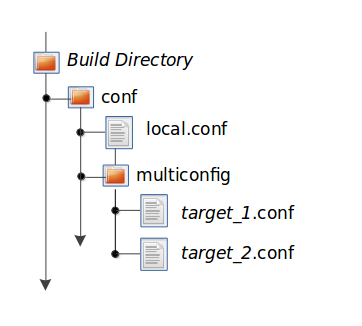
\includegraphics[width=0.4\textwidth]{contents/1_overview/bb_multiconfig_files.png}
\end{center}
The reason for this required file hierarchy is because the \bbgls{BBPATH} variable is not constructed until the layers are parsed. Consequently, using the configuration file as a pre-configuration file is not possible unless it is located in the current working directory.

之所以需要这种文件层次结构,是因为在各个不同的层在被 BitBake 解析之前,\bbgls{BBPATH} 变量不会被正确的构建起来。因此,除非配置文件位于当前工作目录中,否则 BitBake 不可能将其用作预配置文件。

Minimally, each configuration file must define the machine and the temporary directory BitBake uses for the build. Suggested practice dictates that you do not overlap the temporary directories used during the builds.

每个构建配置文件至少要定义目标机器和 BitBake 用于目标机器构建的临时目录。建议的做法是不要将此临时目录与构建期间使用的临时目录重叠。

Aside from separate configuration files for each target, you must also enable BitBake to perform multiple configuration builds. Enabling is accomplished by setting the \bbgls{BBMULTICONFIG} variable in the \code{local.conf} configuration file. As an example, suppose you had configuration files for \code{target1} and \code{target2} defined in the build directory. The following statement in the \code{local.conf} file both enables BitBake to perform multiple configuration builds and specifies the two extra multiconfigs:

除了每个目标有自己的单独构建配置文件之外,你还必须让 BitBake 能够来执行多个配置构建。启用这项功能是通过在构建配置文件中 \code{local.conf} 设置 \bbgls{BBMULTICONFIG} 变量来完成的 。例如,假设你已经在构建目录中为 \code{target1} 和 \code{target2} 定义好了构建配置文件, \code{local.conf} 文件中的以下语句既使 BitBake 能够执行多个配置的构建,又指定了这两个额外的多重配置:

\begin{pyglist}
BBMULTICONFIG = "target1 target2"
\end{pyglist}

Once the target configuration files are in place and BitBake has been enabled to perform multiple configuration builds, use the following command form to start the builds:

一旦目标的构建配置文件准备好了并且 BitBake 已启用以执行多个配置构建,请使用以下命令形式来启动构建工作:

\begin{pyglist}
$ bitbake [mc:multiconfigname:]target [[[mc:multiconfigname:]target] ... ]
\end{pyglist}

Here is an example for two extra multiconfigs: \code{target1} and \code{target2}:

这是两个额外的多重配置的示例:\code{target1} 和 \code{target2}:

\begin{pyglist}
$ bitbake mc::target mc:target1:target mc:target2:target
\end{pyglist}

\newsubsubsection{Enabling Multiple Configuration Build Dependencies}{启用多个配置构建的依赖关系}

Sometimes dependencies can exist between targets (multiconfigs) in a multiple configuration build. For example, suppose that in order to build an image for a particular architecture, the root filesystem of another build for a different architecture needs to exist. In other words, the image for the first multiconfig depends on the root filesystem of the second multiconfig. This dependency is essentially that the task in the recipe that builds one multiconfig is dependent on the completion of the task in the recipe that builds another multiconfig.

有时间多配置构建中的目标(多重配置)之间可能存在相互依赖关系。例如,假设为了构建特定架构的镜像,需要针对不同架构的另一个构建的根文件系统的存在。换句话说,第一个多重配置所构建的镜像是取决于第二个多重配置所构建的根文件系统。这种依赖关系本质上是一个多重配置的配方中的任务的构建是依赖于另一个多重配置的配方中的任务的构建的完成。

To enable dependencies in a multiple configuration build, you must declare the dependencies in the recipe using the following statement form:

要在多配置构建中启用依赖关系向,你必须使用以下语法形式在配方中声明依赖关系项:

\begin{pyglist}
task_or_package[mcdepends] = "mc:from_multiconfig:to_multiconfig:recipe_name:task_on_which_to_depend"
\end{pyglist}

To better show how to use this statement, consider an example with two multiconfigs: \code{target1} and \code{target2}:

为了更好地展示如何使用此语句,请参考下面一个具有两个多重配置的示例:\code{target1} 和 \code{target2}:

\begin{pyglist}
image_task[mcdepends] = "mc:target1:target2:image2:rootfs_task"
\end{pyglist}

In this example, the \code{from_multiconfig} is ``target1'' and the \code{to_multiconfig} is ``target2''. The task on which the image whose recipe contains \code{image_task} depends on the completion of the \code{rootfs_task} used to build out image2, which is associated with the ``target2'' multiconfig.

在此示例中, \code{from_multiconfig} 是 ``target1'',\code{to_multiconfig} 是 ``target2''。配方中包含 \code{image_task} 的镜像所执行的任务取决于用于构建 \code{image2} 的 \code{rootfs_task} 的完成情况,该任务与 ``target2'' 多重配置关联。

Once you set up this dependency, you can build the ``target1'' multiconfig using a BitBake command as follows:

在设置此依赖项后,你可以使用 BitBake 命令来构建 ``target1'' 的多重配置,如下所示:

\begin{pyglist}
$ bitbake mc:target1:image1
\end{pyglist}

This command executes all the tasks needed to create \code{image1} for the ``target1'' multiconfig. Because of the dependency, BitBake also executes through the \code{rootfs_task} for the ``target2'' multiconfig build.

此命令会执行所有为 ``target1''多重构建配置中能够生成 \code{image1} 目标所需的任务。由于依赖关系的存在,BitBake 还会执行 ``target2'' 这个多重配置构建中的 \code{rootfs_task} 任务。

Having a recipe depend on the root filesystem of another build might not seem that useful. Consider this change to the statement in the image1 recipe:

让配方依赖于另一个构建所生成的根文件系统可能看起来并不是那么有用。考虑对 \code{image1} 配方中的语句进行以下更改:

\begin{pyglist}
image_task[mcdepends] = "mc:target1:target2:image2:image_task"
\end{pyglist}

In this case, BitBake must create \code{image2} for the ``target2'' build since the ``target1'' build depends on it.

在这种情况下,BitBake 必须为 ``target2'' 构建生成 \code{image2} 目标,因为 ``target1'' 的构建依赖于它。

Because ``target1'' and ``target2'' are enabled for multiple configuration builds and have separate configuration files, BitBake places the artifacts for each build in the respective temporary build directories.

由于 ``target1'' 和 ``target2'' 已经是被启用的多个配置的构建,并且它们都具有自己单独的配置文件,因此 BitBake 将每个构建的构建生成物都放置在它们各自的临时构建目录中。
